\documentclass[nogin]{beamer}\usepackage[]{graphicx}\usepackage[]{color}
%% maxwidth is the original width if it is less than linewidth
%% otherwise use linewidth (to make sure the graphics do not exceed the margin)
\makeatletter
\def\maxwidth{ %
  \ifdim\Gin@nat@width>\linewidth
    \linewidth
  \else
    \Gin@nat@width
  \fi
}
\makeatother

\definecolor{fgcolor}{rgb}{0.345, 0.345, 0.345}
\newcommand{\hlnum}[1]{\textcolor[rgb]{0.686,0.059,0.569}{#1}}%
\newcommand{\hlstr}[1]{\textcolor[rgb]{0.192,0.494,0.8}{#1}}%
\newcommand{\hlcom}[1]{\textcolor[rgb]{0.678,0.584,0.686}{\textit{#1}}}%
\newcommand{\hlopt}[1]{\textcolor[rgb]{0,0,0}{#1}}%
\newcommand{\hlstd}[1]{\textcolor[rgb]{0.345,0.345,0.345}{#1}}%
\newcommand{\hlkwa}[1]{\textcolor[rgb]{0.161,0.373,0.58}{\textbf{#1}}}%
\newcommand{\hlkwb}[1]{\textcolor[rgb]{0.69,0.353,0.396}{#1}}%
\newcommand{\hlkwc}[1]{\textcolor[rgb]{0.333,0.667,0.333}{#1}}%
\newcommand{\hlkwd}[1]{\textcolor[rgb]{0.737,0.353,0.396}{\textbf{#1}}}%

\usepackage{framed}
\makeatletter
\newenvironment{kframe}{%
 \def\at@end@of@kframe{}%
 \ifinner\ifhmode%
  \def\at@end@of@kframe{\end{minipage}}%
  \begin{minipage}{\columnwidth}%
 \fi\fi%
 \def\FrameCommand##1{\hskip\@totalleftmargin \hskip-\fboxsep
 \colorbox{shadecolor}{##1}\hskip-\fboxsep
     % There is no \\@totalrightmargin, so:
     \hskip-\linewidth \hskip-\@totalleftmargin \hskip\columnwidth}%
 \MakeFramed {\advance\hsize-\width
   \@totalleftmargin\z@ \linewidth\hsize
   \@setminipage}}%
 {\par\unskip\endMakeFramed%
 \at@end@of@kframe}
\makeatother

\definecolor{shadecolor}{rgb}{.97, .97, .97}
\definecolor{messagecolor}{rgb}{0, 0, 0}
\definecolor{warningcolor}{rgb}{1, 0, 1}
\definecolor{errorcolor}{rgb}{1, 0, 0}
\newenvironment{knitrout}{}{} % an empty environment to be redefined in TeX

\usepackage{alltt} %Instead of an article class, use beamer class
\usepackage{graphicx} %Bring in outside images
\usepackage{amssymb,amsmath} %Easy equation typsetter
\usepackage{listings}
\usepackage{colortbl} %More colours
\usetheme{mcgill} % Creates the McGill insignia behind the title page
\usecolortheme[RGB={238,44,44}]{structure}
\usetheme{PaloAlto}
\title{R, Sweave and Beamer}
\author{Christopher Lee}
\setbeamertemplate{itemize items}[ball]
\setbeamertemplate{enumerate items}[circle]
\IfFileExists{upquote.sty}{\usepackage{upquote}}{}

\begin{document}

\frame{\titlepage}

\begin{frame}
\frametitle{Table of Contents}
\tableofcontents
\end{frame}

\begin{frame}[fragile]
\frametitle{Downloading packages}
\footnotesize
\begin{itemize}
\item R is found here:\\
\begin{sloppypar}
\url{http://cran.parentingamerica.com}
\end{sloppypar}
\item For Windows, find either TeX Live or MiKTeX here:
\begin{sloppypar}
\url{http://www.tug.org/texlive/acquire-netinstall.html}
\url{http://miktex.org/download}
\end{sloppypar}
\item For Mac OSX, find  MacTex here:
\begin{sloppypar}
\url{http://tug.org/mactex/}
\end{sloppypar}
\item Beamer should already be preloaded. If not it may be found here:
\begin{sloppypar}
\url{https://bitbucket.org/rivanvx/beamer/wiki/Home}
\end{sloppypar}
\end{itemize}
\end{frame}

\begin{frame}
\frametitle{Online Tutorials}
See the following resources for introductory tutorials and examples for Beamer:
\begin{itemize}
\begin{sloppypar}
\item \url{http://www.math.umbc.edu/~rouben/beamer/}
\item \url{http://www.informatik.uni-freiburg.de/~frank/ENG/latex-course/latex-course-3/latex-course-3_en.html}
\item \url{http://users.stat.umn.edu/~sandy/courses/8801/handouts/03.Beamer/beamer.pdf}
\item \url{http://www.wekaleamstudios.co.uk/supplementary-material/}
\end{sloppypar}
\end{itemize}
\end{frame}

\section{GGPLOT2}
\begin{frame}
\frametitle{Section 1}
\begin{center}
\Large
The Ggplot2 package
\end{center}
\end{frame}

\begin{frame}
\frametitle{Ggplot2}
\begin{block}{Data}
I am using CANSIM 202-0802 data to produce these graphs in R version 3.0.1
\end{block}
Find the data here:\\
\url{http://www.statcan.gc.ca/tables-tableaux/sum-som/l01/cst01/famil41a-eng.htm}
\end{frame}

\begin{frame}[fragile]
\frametitle{Example 1, Line graph}
\begin{knitrout}
\definecolor{shadecolor}{rgb}{0.969, 0.969, 0.969}\color{fgcolor}
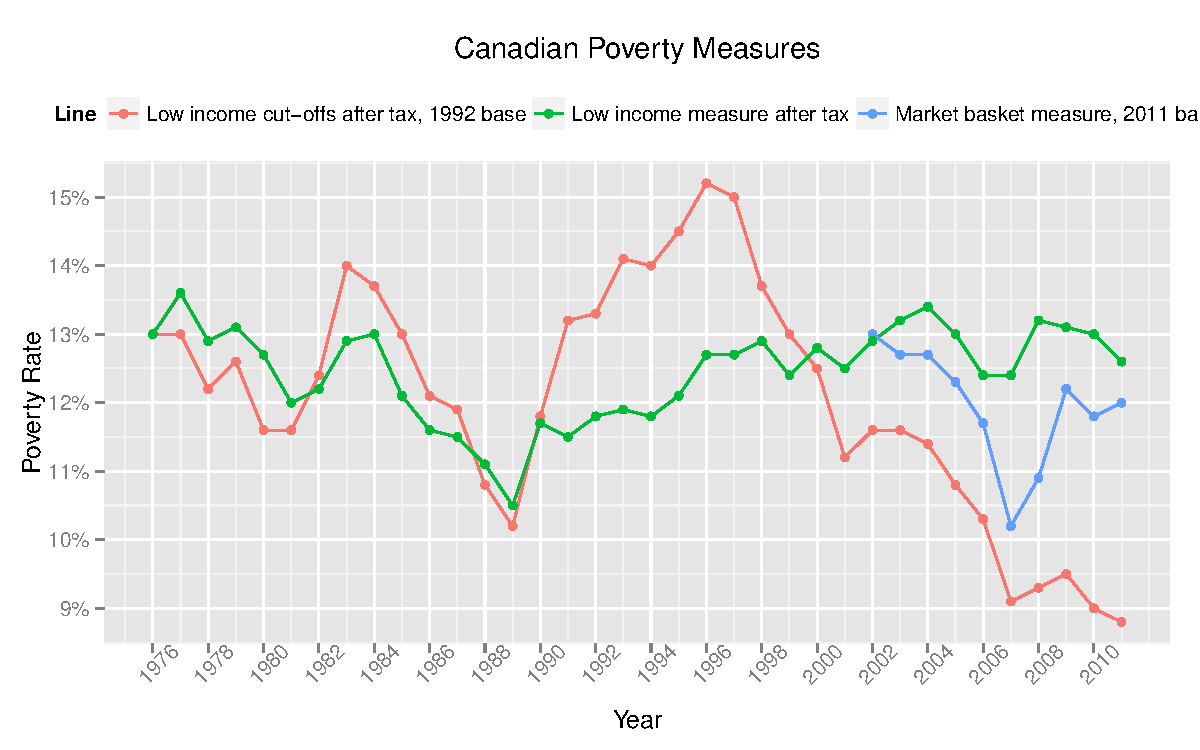
\includegraphics[width=\maxwidth]{figure/unnamed-chunk-1} 

\end{knitrout}

\end{frame}

\begin{frame}[fragile]{Outline}
\frametitle{Example 2, Boxplots}
\begin{knitrout}
\definecolor{shadecolor}{rgb}{0.969, 0.969, 0.969}\color{fgcolor}
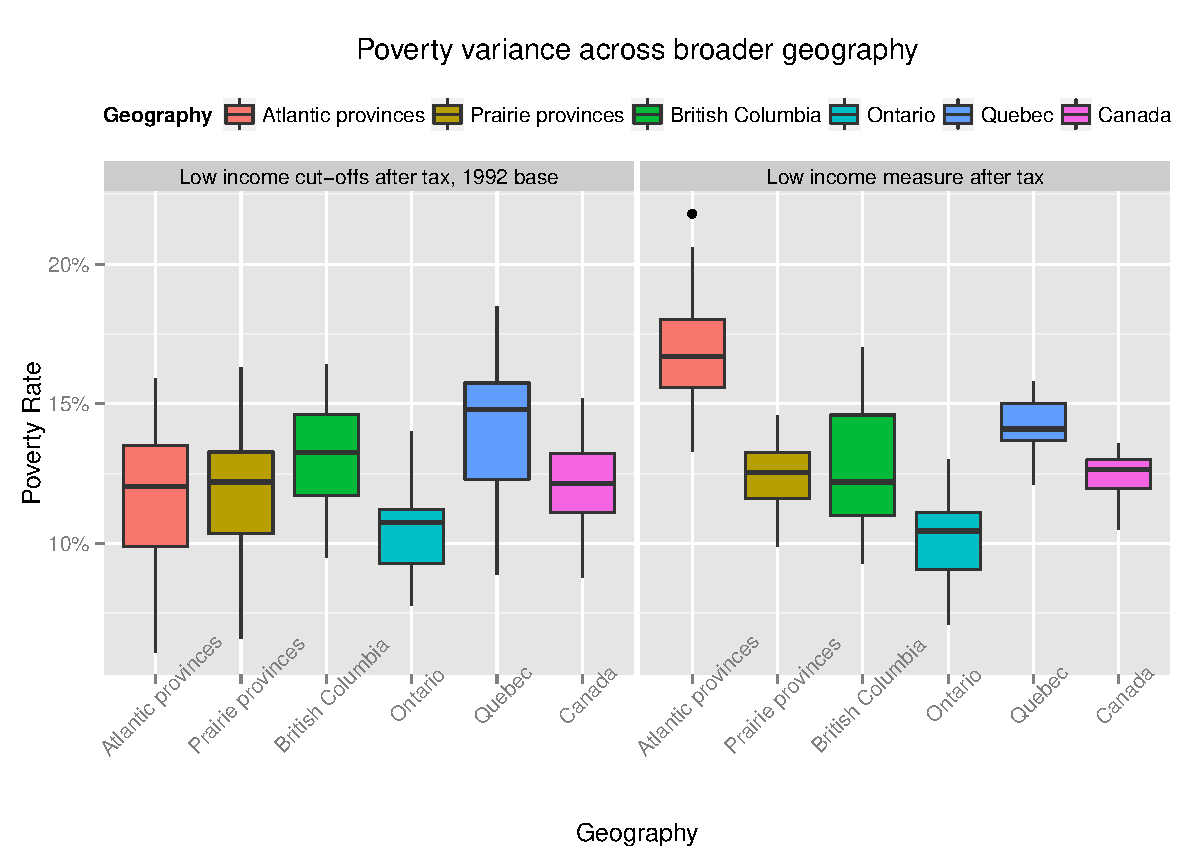
\includegraphics[width=\maxwidth]{figure/unnamed-chunk-2} 

\end{knitrout}

\end{frame}

\begin{frame}[fragile]{Outline}
\frametitle{Example 3 Pie Charts}
\begin{knitrout}
\definecolor{shadecolor}{rgb}{0.969, 0.969, 0.969}\color{fgcolor}
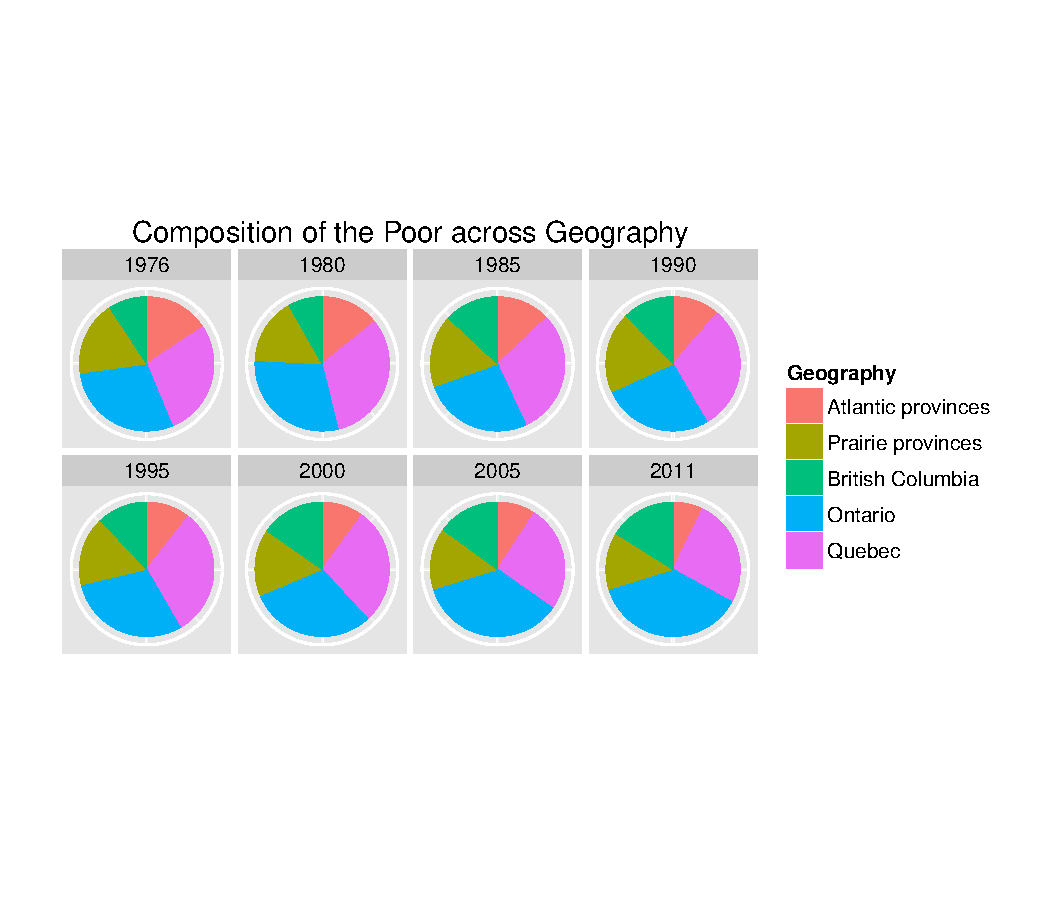
\includegraphics[width=\maxwidth]{figure/unnamed-chunk-3} 

\end{knitrout}

\end{frame}

\begin{frame}[fragile]
\frametitle{GGplot code}
\begin{block}{All these plots start with the same code}
\begin{verbatim}
ggplot(data=DATA,aes(x=X,y=Y,fill=FILL,
                              colour=COLOUR)
\end{verbatim}
\end{block}
\footnotesize
\begin{columns}[T]
\begin{column}{0.5\textwidth}
\begin{itemize}
\item DATA = self explanatory, our dataframe
\item X = What we want to plot on the x-axis
\item Y = What we want to plot on the y-axis
\item FILL = For our 3rd variable to create sections/bins ontop of the x and y axes.
\end{itemize}
\end{column}
\begin{column}{0.5\textwidth}
\begin{itemize}
\item COLOUR = Similar to FILL, it is created to map a third variable onto the plot.
\item Notice, this alone is not sufficient to create a plot. We have specified the parameters, but now must specify what type of plot we want
\end{itemize}
\end{column}
\end{columns}
\end{frame}

\begin{frame}[fragile]
\frametitle{Geom code}
\begin{block}{Geom line, Geom boxplot, Geom point, Geom bar}
Here we pick which plots we want to use. Many arguments within the geom functions are very similar to the ones in the ggplot argument. Notice, if you have correctly specified your  x, y and the third variable, you can leave \verb|geom_()| blank
\end{block}
\begin{itemize}
\item 
\begin{verbatim}geom_line() :             Line graph
\end{verbatim}
\item
\begin{verbatim}geom_boxplot() :          Side-by-side \end{verbatim}
\begin{verbatim}                          boxplots
\end{verbatim}
\item
\begin{verbatim}geom_bar(stat='identity) : Bar charts/\end{verbatim}
\begin{verbatim}                          histogram
\end{verbatim}
\item
\begin{verbatim}geom_area() :             Area plot
\end{verbatim}
\end{itemize}
\end{frame}

\begin{frame}[fragile]
\frametitle{Miscallaneous code}
Now with our plots we can tidy up the labels, axes, scales and legends
\scriptsize
\begin{columns}[T]
\begin{column}{0.5\textwidth}
\begin{block}{Imputs}
\begin{itemize}
\item \begin{verbatim} ylab \end{verbatim}
\item \begin{verbatim} xlab \end{verbatim}
\item \begin{verbatim} ggtitle \end{verbatim}
\item \begin{verbatim} guides \end{verbatim}
\item \begin{verbatim} theme \end{verbatim}
\item \begin{verbatim} scale_y_continuous \end{verbatim}
\item \begin{verbatim} scale_x_discrete \end{verbatim}
\end{itemize}
\end{block}
\end{column}
\begin{column}{0.5\textwidth}
\begin{block}{Explanation}
\begin{itemize}
\item Title for y-axis
\item Title for x-axis
\item Main Title
\item Controls legend
\item Remove or angle ticks
\item Control y-axis breaks and ticks
\item Contrl x-axis breaks and ticks
\end{itemize}
\end{block}
\end{column}
\end{columns}
\end{frame}

\begin{frame}[fragile]
\frametitle{Example output}
\begin{knitrout}
\definecolor{shadecolor}{rgb}{0.969, 0.969, 0.969}\color{fgcolor}
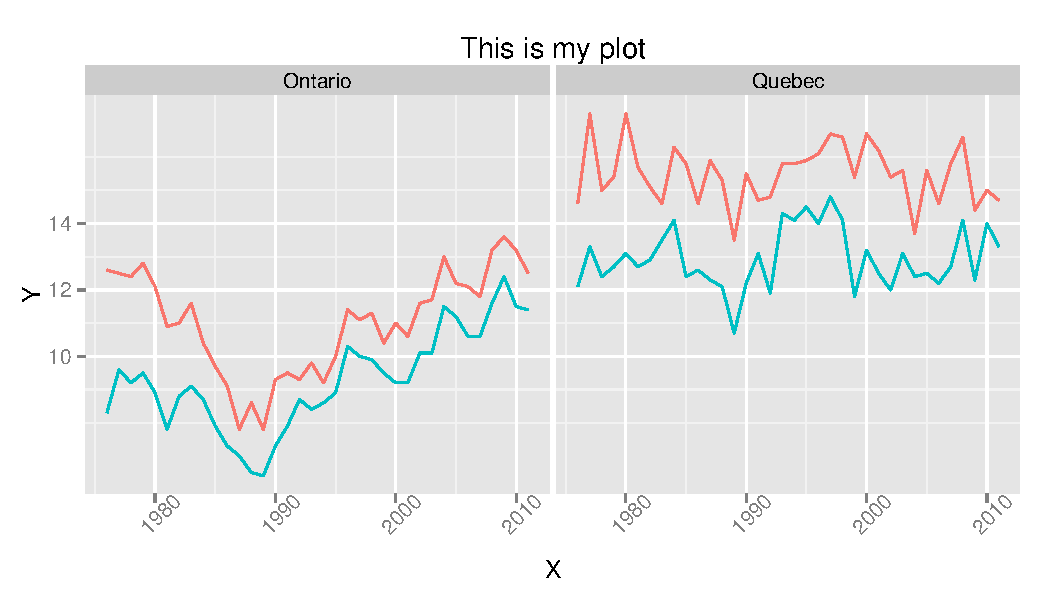
\includegraphics[width=\maxwidth]{figure/unnamed-chunk-4} 

\end{knitrout}

\end{frame}

\begin{frame}[fragile]
\frametitle{Example code explanation}
\scriptsize
From our dataset DATA, we graph the variable \emph{Year} on the x-axis and the variable \emph{Value} on the y-axis. We assign a seperate color for every  factor level of the variable \emph{Population}.
\begin{verbatim}ggplot(data=DATA,aes(x=Year,y=Value,colour=Population))+\end{verbatim}
We specify that we want a line graph, and title the plot.
\begin{verbatim}geom_line()+gggtitle("This is my plot")\end{verbatim}
We title the y-axis \emph{Y} and the x-axis {X}. We also suppress the legend.
\begin{verbatim}ylab("Pov. rates")+xlab("Time")+guides(fill=FALSE)+\end{verbatim}
We control the y-axis and create ticks on the numbers 10, 12 and 14 of the variable \emph{Value}.
\begin{verbatim}scale_y_continuous(breaks=c(10,12,14))+ \end{verbatim}
We control the tick labels on the x-axis. We angle the tick labels 45 degrees
\begin{verbatim}theme(axis.text.x=element_text(angle=45))+
\end{verbatim}
We create several of these plots, each using a different factor level from the variable \emph{Geography}. Essentially, each plot is using different data according to a unique value of \emph{Geography}
\begin{verbatim}facet_grid(.~Geography)\end{verbatim}
\end{frame}

\begin{frame}
\frametitle{Result}
The graphic is now ready to be placed into a LaTeX environment. No additional wrapper is necessary to bring this graphic from R into LaTeX and eventually to exportable .pdf. We will reuse this code later.
\end{frame}

\begin{frame}[fragile]
\frametitle{Other resources}
For more information see the following links
\begin{itemize}
\item \url{http://www.cookbook-r.com/Graphs/}
\item \url{http://sharpstatistics.co.uk/r/ggplot2-guide/}
\item \url{http://www.ceb-institute.org/bbs/wp-content/uploads/2011/09/handout_ggplot2.pdf}
\end{itemize}
\end{frame}

\section{Xtable and Hmisc}
\begin{frame}
\frametitle{Section 2}
\begin{center}
\Large
Exporting Tables to LaTeX environments
\end{center}
\end{frame}

\begin{frame}[fragile]
\frametitle{Xtable and Hmisc}
\begin{block}{Now what about tables?}
We've seen how to create graphics and plots using ggplot within R. Now lets see how to create tables ready to be exported into LaTeX. There are two packages in R designed for this. To use either, imput the following two lines of code
\begin{enumerate}
\item Xtable
\begin{verbatim}install.packages("xtable")
library(xtable)\end{verbatim}
\item Hmisc
\begin{verbatim}install.packages("Hmisc")
library(Hmisc)\end{verbatim}
\end{enumerate}
\end{block}
\end{frame}

\begin{frame}[fragile]
\frametitle{Exporting R tables as LaTeX tables }
\begin{itemize}
\item Tables are only slightly more tricky than plots, in that there are several base R functions to summarize data and create tables in the console. But that output is not immediately exportable to LaTeX
\item We look to Xtable and Hmisc, which allows us to wrap R tables within a function that translates it into LaTeX code.
\item Exportable objects can range from contingency tables to matrices, regression summaries, ANOVA tables and even raw data
\end{itemize}
\end{frame}

\begin{frame}
\frametitle{Xtable}
\begin{block}{Exporting using Xtable}
I generally prefer Xtable to Hmisc because
\begin{enumerate}
\item xtable can wrap tables from almost all objects and classes
\item You can modify the LaTeX output a great deal in xtable
\item Most importantly, xtable can export tables without a float
\end{enumerate}
More on the float environment later.
\end{block}
\end{frame}

\begin{frame}[fragile]
\frametitle{List of base tables}
\begin{columns}[T]
\begin{column}{.5\textwidth}
\begin{block}{R function}
\begin{itemize}
\item \begin{verbatim}table()\end{verbatim}
\item \begin{verbatim}xtabs()\end{verbatim}
\item \begin{verbatim}prop.table()\end{verbatim}
\item \begin{verbatim}aggregate()\end{verbatim}
\item \begin{verbatim}anova()\end{verbatim}
\end{itemize}
\end{block}
\end{column}
\begin{column}{.5\textwidth}
\begin{block}{Description}
\begin{itemize}
\footnotesize
\item 2-way contingency table
\item 3-way contingency table
\item 2-way frequency table
\item Custom aggregate data
\item Analysis of variance wrapper around a regression object
\end{itemize}
\end{block}
\end{column}
\end{columns}
\end{frame}

\begin{frame}[fragile,shrink]
\frametitle{Xtable imput}
\begin{block}{}
Take nearly any R object of class dataframe, matrix, array, aov, lm...\\
and then enter \verb|xtable(x)| to provide LaTeX output. You are given a series of options for the output.
\end{block}
\begin{columns}[T]
\begin{column}{.5\textwidth}
\begin{itemize}
\item Digits
\item Line divisions
\item Floating environment
\end{itemize}
\end{column}
\begin{column}{.5\textwidth}
\begin{itemize}
\item Captions
\item Alignment of columns
\item and more
\end{itemize}
\end{column}
\end{columns}
\end{frame}

\begin{frame}[fragile,shrink]
\frametitle{Wrapping xtable in print}
\small
Wrapping xtable in the print function is essential because it allows us to specify the LaTeX object to not float the table. A floated table is within a table environment and is sandwiched between \verb|\begin{table}| and \verb|\end{table}|\\[\baselineskip]
Once a table is floated there is very little we can do with it. The biggest problem is always \textbf{Overfull Hbox}. Tables are often too long to fit to the page width. Since Beamer is in a presentation format, its a bad idea to play around too much with the page size.\\[\baselineskip]

Sometimes we have Overfull Vbox where the table is too long, but this is easily corrected by specifying xtable to deliver output in "longtable" format and splitting the table across multiple frames. This cannot be done with wide tables. 
\end{frame}

\begin{frame}[fragile]
\frametitle{Wrapping xtable in print Cont...}
We can shrink this "un-floated" table by first loading the \textbf{graphicx} package into LaTeX and then use the \textbf{resize} argument. It should look something like this.
\begin{verbatim}
\documentclass{beamer}
\usepackage{graphicx}
\begin{document}
\resizebox{\linewidth}{!}{%
<<echo=FALSE,warning=FALSE>> =
print(xtable(x),floating=FALSE)
@
}
\end{verbatim}
\end{frame}

\begin{frame}[fragile,shrink]
\frametitle{Xtable example part 1}
First lets create the table in R. It doesn't look too nice.
\begin{verbatim}table<-with(subset(data2,data2$Year>=2000&data2$Geography=="Canada"&
data2$Statistic=="Percentage of persons in low income"&
as.character(data2$Line)=="Low income cut-offs after tax, 1992 base"),
xtabs(Value~Population+Year))
\end{verbatim}
\begin{knitrout}
\definecolor{shadecolor}{rgb}{0.969, 0.969, 0.969}\color{fgcolor}\begin{kframe}
\begin{verbatim}
##                                  Year
## Population                        2000 2001 2002 2003 2004 2005 2006 2007
##   Females                         13.6 12.1 12.4 12.2 11.9 11.1 10.7  9.3
##   Males                           11.4 10.3 10.7 11.0 10.8 10.5 10.0  9.0
##   Persons under 18 years          13.9 12.2 12.4 12.7 13.0 11.7 11.1  9.5
##   Persons 18 to 64 years          12.9 11.7 12.0 12.2 11.9 11.4 11.1  9.9
##   Persons 65 years and over        7.6  6.7  7.6  6.8  5.6  6.2  5.3  4.8
##   Persons in economic families     9.3  8.1  8.6  8.7  8.2  7.5  7.1  6.0
##   Child in single mother families 40.1 37.4 43.0 41.4 40.4 32.9 31.2 26.7
##   Child in two-parent families     9.5  8.3  7.4  7.9  8.4  7.8  7.5  6.5
##   Unattached individuals          32.9 30.8 29.5 29.7 30.1 30.5 29.4 27.6
##   All persons                     12.5 11.2 11.6 11.6 11.4 10.8 10.3  9.1
##                                  Year
## Population                        2008 2009 2010 2011
##   Females                          9.8  9.5  9.3  8.9
##   Males                            8.9  9.5  8.7  8.7
##   Persons under 18 years           9.0  9.4  8.2  8.5
##   Persons 18 to 64 years          10.1 10.4 10.1  9.7
##   Persons 65 years and over        5.8  5.1  5.3  5.2
##   Persons in economic families     6.2  6.5  5.9  5.5
##   Child in single mother families 23.3 21.5 21.8 23.0
##   Child in two-parent families     6.4  7.3  5.7  5.9
##   Unattached individuals          27.3 26.9 26.9 27.7
##   All persons                      9.3  9.5  9.0  8.8
\end{verbatim}
\end{kframe}
\end{knitrout}

\end{frame}

\begin{frame}[fragile]
\frametitle{Xtable example part 2}
Now lets wrap our xtab() table within xtable.
\begin{verbatim}
table2<-
xtable(table,digits=1,align="l|rrrrrrrrrrrr")
\end{verbatim}
\begin{knitrout}
\definecolor{shadecolor}{rgb}{0.969, 0.969, 0.969}\color{fgcolor}\begin{kframe}
\begin{verbatim}
## % latex table generated in R 3.0.1 by xtable 1.7-1 package
## % Wed Jan  8 10:22:00 2014
## \begin{table}[ht]
## \centering
## \begin{tabular}{l|rrrrrrrrrrrr}
##   \hline
##  & 2000 & 2001 & 2002 & 2003 & 2004 & 2005 & 2006 & 2007 & 2008 & 2009 & 2010 & 2011 \\ 
##   \hline
## Females & 13.6 & 12.1 & 12.4 & 12.2 & 11.9 & 11.1 & 10.7 & 9.3 & 9.8 & 9.5 & 9.3 & 8.9 \\ 
##   Males & 11.4 & 10.3 & 10.7 & 11.0 & 10.8 & 10.5 & 10.0 & 9.0 & 8.9 & 9.5 & 8.7 & 8.7 \\ 
##   Persons under 18 years & 13.9 & 12.2 & 12.4 & 12.7 & 13.0 & 11.7 & 11.1 & 9.5 & 9.0 & 9.4 & 8.2 & 8.5 \\ 
##   Persons 18 to 64 years & 12.9 & 11.7 & 12.0 & 12.2 & 11.9 & 11.4 & 11.1 & 9.9 & 10.1 & 10.4 & 10.1 & 9.7 \\ 
##   Persons 65 years and over & 7.6 & 6.7 & 7.6 & 6.8 & 5.6 & 6.2 & 5.3 & 4.8 & 5.8 & 5.1 & 5.3 & 5.2 \\ 
##   Persons in economic families & 9.3 & 8.1 & 8.6 & 8.7 & 8.2 & 7.5 & 7.1 & 6.0 & 6.2 & 6.5 & 5.9 & 5.5 \\ 
##   Child in single mother families & 40.1 & 37.4 & 43.0 & 41.4 & 40.4 & 32.9 & 31.2 & 26.7 & 23.3 & 21.5 & 21.8 & 23.0 \\ 
##   Child in two-parent families & 9.5 & 8.3 & 7.4 & 7.9 & 8.4 & 7.8 & 7.5 & 6.5 & 6.4 & 7.3 & 5.7 & 5.9 \\ 
##   Unattached individuals & 32.9 & 30.8 & 29.5 & 29.7 & 30.1 & 30.5 & 29.4 & 27.6 & 27.3 & 26.9 & 26.9 & 27.7 \\ 
##   All persons & 12.5 & 11.2 & 11.6 & 11.6 & 11.4 & 10.8 & 10.3 & 9.1 & 9.3 & 9.5 & 9.0 & 8.8 \\ 
##    \hline
## \end{tabular}
## \end{table}
\end{verbatim}
\end{kframe}
\end{knitrout}

\end{frame}

\begin{frame}[fragile]
\frametitle{Example part 3}
We have to modify our R chunk code for LaTeX to properly read xtable
\begin{verbatim}
<<echo=FALSE,warning=FALSE, results='asis'>> =
table2<-
xtable(table,digits=1,align="l|rrrrrrrrrrrr")
@
\end{verbatim}
% latex table generated in R 3.0.1 by xtable 1.7-1 package
% Wed Jan  8 10:22:00 2014
\begin{table}[ht]
\centering
\begin{tabular}{l|rrrrrrrrrrrr}
  \hline
 & 2000 & 2001 & 2002 & 2003 & 2004 & 2005 & 2006 & 2007 & 2008 & 2009 & 2010 & 2011 \\ 
  \hline
Females & 13.6 & 12.1 & 12.4 & 12.2 & 11.9 & 11.1 & 10.7 & 9.3 & 9.8 & 9.5 & 9.3 & 8.9 \\ 
  Males & 11.4 & 10.3 & 10.7 & 11.0 & 10.8 & 10.5 & 10.0 & 9.0 & 8.9 & 9.5 & 8.7 & 8.7 \\ 
  Persons under 18 years & 13.9 & 12.2 & 12.4 & 12.7 & 13.0 & 11.7 & 11.1 & 9.5 & 9.0 & 9.4 & 8.2 & 8.5 \\ 
  Persons 18 to 64 years & 12.9 & 11.7 & 12.0 & 12.2 & 11.9 & 11.4 & 11.1 & 9.9 & 10.1 & 10.4 & 10.1 & 9.7 \\ 
  Persons 65 years and over & 7.6 & 6.7 & 7.6 & 6.8 & 5.6 & 6.2 & 5.3 & 4.8 & 5.8 & 5.1 & 5.3 & 5.2 \\ 
  Persons in economic families & 9.3 & 8.1 & 8.6 & 8.7 & 8.2 & 7.5 & 7.1 & 6.0 & 6.2 & 6.5 & 5.9 & 5.5 \\ 
  Child in single mother families & 40.1 & 37.4 & 43.0 & 41.4 & 40.4 & 32.9 & 31.2 & 26.7 & 23.3 & 21.5 & 21.8 & 23.0 \\ 
  Child in two-parent families & 9.5 & 8.3 & 7.4 & 7.9 & 8.4 & 7.8 & 7.5 & 6.5 & 6.4 & 7.3 & 5.7 & 5.9 \\ 
  Unattached individuals & 32.9 & 30.8 & 29.5 & 29.7 & 30.1 & 30.5 & 29.4 & 27.6 & 27.3 & 26.9 & 26.9 & 27.7 \\ 
  All persons & 12.5 & 11.2 & 11.6 & 11.6 & 11.4 & 10.8 & 10.3 & 9.1 & 9.3 & 9.5 & 9.0 & 8.8 \\ 
   \hline
\end{tabular}
\end{table}


\end{frame}

\begin{frame}[fragile]
\frametitle{Example part 4}
Now you see our Overfull Hbox problem. First we wrap the xtable within print, specify floating=FALSE and resize the table
\begin{verbatim}
\resizebox{\linewidth}{!}{%
<<echo=FALSE,warning=FALSE,results='asis'>> =
print(table2,floating=FALSE)
@
}
\end{verbatim}
\resizebox{\linewidth}{!}{%
% latex table generated in R 3.0.1 by xtable 1.7-1 package
% Wed Jan  8 10:22:00 2014
\begin{tabular}{l|rrrrrrrrrrrr}
  \hline
 & 2000 & 2001 & 2002 & 2003 & 2004 & 2005 & 2006 & 2007 & 2008 & 2009 & 2010 & 2011 \\ 
  \hline
Females & 13.6 & 12.1 & 12.4 & 12.2 & 11.9 & 11.1 & 10.7 & 9.3 & 9.8 & 9.5 & 9.3 & 8.9 \\ 
  Males & 11.4 & 10.3 & 10.7 & 11.0 & 10.8 & 10.5 & 10.0 & 9.0 & 8.9 & 9.5 & 8.7 & 8.7 \\ 
  Persons under 18 years & 13.9 & 12.2 & 12.4 & 12.7 & 13.0 & 11.7 & 11.1 & 9.5 & 9.0 & 9.4 & 8.2 & 8.5 \\ 
  Persons 18 to 64 years & 12.9 & 11.7 & 12.0 & 12.2 & 11.9 & 11.4 & 11.1 & 9.9 & 10.1 & 10.4 & 10.1 & 9.7 \\ 
  Persons 65 years and over & 7.6 & 6.7 & 7.6 & 6.8 & 5.6 & 6.2 & 5.3 & 4.8 & 5.8 & 5.1 & 5.3 & 5.2 \\ 
  Persons in economic families & 9.3 & 8.1 & 8.6 & 8.7 & 8.2 & 7.5 & 7.1 & 6.0 & 6.2 & 6.5 & 5.9 & 5.5 \\ 
  Child in single mother families & 40.1 & 37.4 & 43.0 & 41.4 & 40.4 & 32.9 & 31.2 & 26.7 & 23.3 & 21.5 & 21.8 & 23.0 \\ 
  Child in two-parent families & 9.5 & 8.3 & 7.4 & 7.9 & 8.4 & 7.8 & 7.5 & 6.5 & 6.4 & 7.3 & 5.7 & 5.9 \\ 
  Unattached individuals & 32.9 & 30.8 & 29.5 & 29.7 & 30.1 & 30.5 & 29.4 & 27.6 & 27.3 & 26.9 & 26.9 & 27.7 \\ 
  All persons & 12.5 & 11.2 & 11.6 & 11.6 & 11.4 & 10.8 & 10.3 & 9.1 & 9.3 & 9.5 & 9.0 & 8.8 \\ 
   \hline
\end{tabular}


}
\end{frame}

\begin{frame}
\frametitle{Floating}
Remember, the \textbf{resize} command will only work on a "non-floating" object. Therefore if you have an Overfull hbox, you must first wrap your table in print() and specify floating=FALSE.\\[\baselineskip]
I'll go over the R chunk code and Sweave code in the next section.
\end{frame}

\begin{frame}[fragile]
\frametitle{A simpler solution: Xtable font size}
Sometimes the resize command is unecessary and a simpler solution is available. Xtable allows for us to change the font size from normal size to {\tiny very small} to {\Large very large}
\begin{block}{xtable(...,size="  ")}
By changing the font size of the table, we can easily remedy minor Overfull Hbox and Vbox. There are 10 sizes.
\begin{columns}[T]
\begin{column}{.25\linewidth}
\begin{itemize}
\item {\tiny tiny}
\item {\scriptsize scriptsize}
\item {\footnotesize footnotesize}
\item {\small small}
\end{itemize}
\end{column}
\begin{column}{.25\linewidth}
\begin{itemize}
\item {\normalsize normal}
\item {\large large}
\item {\Large Large}
\end{itemize}
\end{column}
\begin{column}{.5\linewidth}
\begin{itemize}
\item {\LARGE LARGE}
\item {\huge huge}
\item {\Huge Huge}
\end{itemize}
\end{column}
\end{columns}
\end{block}
\end{frame}

\begin{frame}[fragile]
\small
\frametitle{Dressing up a table}
Lets say we have a properly sized vanilla table
\begin{columns}[T]
\begin{column}{0.5\textwidth}
% latex table generated in R 3.0.1 by xtable 1.7-1 package
% Wed Jan  8 10:22:00 2014
\begin{table}[ht]
\centering
\begin{tabular}{rrrr}
  \hline
 & LICO & LIM & MBM \\ 
  \hline
1995 & 14.50 & 12.10 &  \\ 
  1996 & 15.20 & 12.70 &  \\ 
  1997 & 15.00 & 12.70 &  \\ 
  1998 & 13.70 & 12.90 &  \\ 
  1999 & 13.00 & 12.40 &  \\ 
  2000 & 12.50 & 12.80 &  \\ 
  2001 & 11.20 & 12.50 &  \\ 
  2002 & 11.60 & 12.90 & 13.00 \\ 
  2003 & 11.60 & 13.20 & 12.70 \\ 
  2004 & 11.40 & 13.40 & 12.70 \\ 
  2005 & 10.80 & 13.00 & 12.30 \\ 
  2011 & 8.80 & 12.60 & 12.00 \\ 
   \hline
\end{tabular}
\end{table}


\end{column}
\begin{column}{0.45\textwidth}
We will try to add a few features to the table:
\begin{itemize}
\item Percentage signs
\item Captions
\item Line divisions
\item A little colour
\end{itemize}
To use the following code add \verb|\usepackage{colortbl}| to the preamble and \verb|library(stringr)| to the chunk code
\end{column}
\end{columns}
\end{frame}

\begin{frame}[fragile]
\frametitle{Dressing up a table: Result}
\begin{columns}[T]
\begin{column}{.5\textwidth}
% latex table generated in R 3.0.1 by xtable 1.7-1 package
% Wed Jan  8 10:22:00 2014
\begin{table}[ht]
\centering
{\small
\begin{tabular}{l||c|c|c}
  \rowcolor[rgb]{1,.8,.8} \hline
 & LICO & LIM & MBM \\ 
  \hline
1995 & 14.5\% & 12.1\% &  \\ 
   \rowcolor[gray]{.9}1996 & 15.2\% & 12.7\% &  \\ 
  1997 & 15.0\% & 12.7\% &  \\ 
   \rowcolor[gray]{.9}1998 & 13.7\% & 12.9\% &  \\ 
  1999 & 13.0\% & 12.4\% &  \\ 
   \rowcolor[gray]{.9}2000 & 12.5\% & 12.8\% &  \\ 
  2001 & 11.2\% & 12.5\% &  \\ 
   \rowcolor[gray]{.9}2002 & 11.6\% & 12.9\% & 13.0\% \\ 
   \rowcolor[rgb]{.8,1,0}2003 & 11.6\% & 13.2\% & 12.7\% \\ 
   \rowcolor[gray]{.9}2004 & 11.4\% & 13.4\% & 12.7\% \\ 
  2005 & 10.8\% & 13.0\% & 12.3\% \\ 
   \rowcolor[gray]{.9} \hline
2011 & 8.8\% & 12.6\% & 12.0\% \\ 
   \hline
\end{tabular}
}
\caption{Poverty Lines} 
\end{table}


\end{column}
\begin{column}{.45\textwidth}
\scriptsize
\begin{lstlisting}
tab3<-apply(tab2, 2, func)
func<-function(u){
  ifelse(!is.na(u),
  sprintf("%.1f%%",u),u)}
pos<-as.list(seq(1,
 nrow(tab3),by=2))
com<-rep(
  "\\rowcolor[gray]{.9}",
 length(pos))
print(xtable(tab3,
   caption="Poverty Lines",
   align="l||c|c|c",
   size="small"),
  hline.after=
   c(-1,0,11,nrow(tab2)),
  add.to.row=list(
   pos=c(list(-1,8),pos),
   command=c(
    "\\rowcolor[rgb]{1,.8,.8}",
    "\\rowcolor[rgb]{.8,1,0}",
    com)))
\end{lstlisting}
\end{column}
\end{columns}
\end{frame}
\begin{frame}[fragile]
\frametitle{Dressing up a table: Explanation}
\footnotesize
First we define a function that will paste a \% on every non-NA element
\begin{verbatim}
  tab3<-apply(tab2, 2, function(u) 
    ifelse(!is.na(u),sprintf( "%.1f%%", u),u))
\end{verbatim}
Then we need to specify the rows in the table which are alternating
\begin{verbatim}
  pos<-as.list(seq(1,nrow(tab3),by=2))
\end{verbatim}
Then we pick the color for the alternating rows defined by \verb|pos|
\begin{verbatim}
  com<-rep("\\rowcolor[gray]{.9}",length(pos))
\end{verbatim}
Now call xtable and use the caption option to define your caption
\begin{verbatim}
  print(xtable(tab3,caption="Poverty Lines",
\end{verbatim}
Create vertical lines between certain columns
\begin{verbatim}
  align="l||c|c|c",
\end{verbatim}
Also specify a different font size for the table and close xtable options
\begin{verbatim}
  size="small"),
\end{verbatim}
\end{frame}
\begin{frame}[fragile]
\frametitle{Dressing up a table: Explanation cont.}
\footnotesize
Now in the print options, create horizontal lines to divide key rows
\begin{verbatim}
  hline.after=c(-1,0,11,nrow(tab2)),
\end{verbatim}
Select the header, another row and our alternating rows
\begin{verbatim}
  add.to.row=list(pos=c(list(-1,8),pos),
\end{verbatim}
Now lets select colors for these select rows
\begin{verbatim}
  command=c("\\rowcolor[rgb]{1,.8,.8}",
    "\\rowcolor[rgb]{.8,1,0}",
    com)))
\end{verbatim}
Now we are finished.
\end{frame}

\begin{frame}[fragile]
\frametitle{A few things on Hmisc}
The Hmisc equivalent of the \verb|xtable()| wrapper  is the \verb|latex()| function. To my knowledge, \verb|latex()| will always float the output. So in cases of Overfull Hbox, the table cannot be resized to fit the page.\\[\baselineskip]
If you do not run into a Overfull Hbox, there are cool features in Hmisc not available in xtable, mainly its summarize.formula functions which will only work with Hmisc's latex wrapper
\end{frame}

\section{Sweave}
\begin{frame}
\frametitle{Section 3}
\begin{center}
\Large
Using Sweave and Knitr
\end{center}
\end{frame}

\begin{frame}
\frametitle{Sweave and Knitr}
Now knowing how to create plots and tables in a LaTeX format, how exacty do we get our R code into LaTeX in the first place? The generic R script file will not work. To get started
\begin{itemize}
\item Open R
\item Instead of a script file, open up an R Sweave file with extension .Rnw
\item Go to Tools $\Rightarrow$ Options $\Rightarrow$ Sweave
\item Select  "Weave Rnw files using" $\Rightarrow$ knitr
\end{itemize}
You must have LaTeX in order to run this type of file. We will use \textbf{knitr} to move R code into LaTeX code, rather than the default \textbf{Sweave} which has a few annoying problems
\end{frame}

\begin{frame}[fragile]
\frametitle{Sweave layout}
\begin{block}{}
In a .Rnw file, you must use LaTeX code. To use R code instead, you must create a "Chunk".
\end{block}
\begin{columns}[T]
\begin{column}{.5\textwidth}
\begin{itemize}
\item To begin the chunk, type:
\begin{verbatim}<<>>=\end{verbatim}
\item To end the chunk, type:
\begin{verbatim}@\end{verbatim}
\end{itemize}
\end{column}
\begin{column}{.5\textwidth}
On your screen it should look like this:
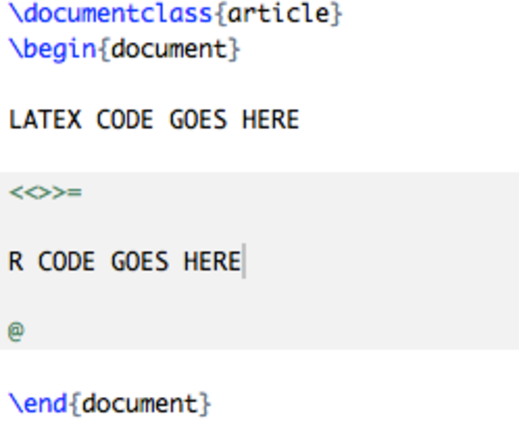
\includegraphics[width=\textwidth]{GuidePic1.pdf}
\end{column}\end{columns}
\end{frame}

\begin{frame}[fragile]
\frametitle{R to Sweave}
\begin{itemize}
\item Within the chunk, the R code is exactly the same as if you were writing R code in a script file.
\item It is better to create a chunk for every table or plot, rather than putting all your R code and figures/tables in the same chunk.
\item Plots are almost never sized correctly to the page. You will have to tweak with the chunk code in order to display plots with your desired dimensions.
\end{itemize}
\end{frame}

\begin{frame}[fragile]
\frametitle{Chunk Code}
\scriptsize
You can control the output of the R code within your chunk.
\begin{verbatim} << options go here >>= \end{verbatim}
A couple options:
\begin{columns}[T]
\begin{column}{.3\textwidth}
\begin{itemize}
\item echo
\item warnings
\item results
\item include
\item size
\item message
\item fig.height
\item fig.width
\end{itemize}
\end{column}
\begin{column}{.7\textwidth}
\begin{itemize}
\item Prints the R code in the output
\item Prints the warnings in the output
\item Whether to display the chunk output
\item How to display the chunk output
\item Font size of chunk output
\item Prints messages in the output
\item Change height of figure
\item Change width of figure
\end{itemize}
\end{column}
\end{columns}
\end{frame}

\begin{frame}[fragile]
\frametitle{Chunk code example}
\begin{verbatim}<<echo=FALSE,warning=FALSE,message=FALSE,
                  fig.height=4,size='tiny'>>=\end{verbatim}
\begin{itemize}
\item The actual R chunk code is not displayed
\item Warnings from the R chunk code are not displayed
\item Messages from the R chunk code are not displayed
\item The figure in the chunk has a height of 4 inches
\item The font size for the chunk output is {\tiny tiny}
\end{itemize}
\end{frame}

\begin{frame}
\frametitle{Finally, compiling the .pdf}
\begin{itemize}
\item After you have set up your R chunk with LaTeX friendly plots and tables, the very last step is to click \textbf{Compile PDF}
\item This will create several files, a .log file, a .tex file, several auxilary files and the .pdf file.
\item Any plot output from your R chunks will also be saved in a folder (if unspecified) called \textbf{figure} in whichever directory you are working from.
\end{itemize}
\end{frame}

\section{Beamer}
\begin{frame}
\frametitle{Section 3}
\begin{center}
\Large
Beamer and LaTeX
\end{center}
\end{frame}

\begin{frame}[fragile]
\frametitle{LaTeX Preamble}
Here's a very basic intro to LaTeX for the purposes of Beamer.
\begin{enumerate}
\item Define a document class. We want beamer
\item Run any packages you require for LaTeX
\item Choose your desired beamer color and theme
\item Create a title
\item Create an author
\item Run any other beamer options
\end{enumerate}
\end{frame}

\begin{frame}[fragile]
\frametitle{LaTeX Preamble example}
\begin{enumerate}
\item \verb|\documentclass{beamer}|
\item \verb|\usepackage{graphicx}|
\item \verb|\usetheme{PaloAlto}|
\item \verb|\title{This is my title}|
\item \verb|\author{This is my name}|
\item \verb|\setbeamertemplate{itemize items}[ball]|
\end{enumerate}
\end{frame}

\begin{frame}[fragile]
\frametitle{Title and ToC}
Now that the preamble is finished, lets get onto the code:
\begin{enumerate}
\item \verb|\begin{document}|
\item \verb|\frame{\titlepage}|
\item \verb|\tableofcontents|
\end{enumerate}
\begin{itemize}
\item No. 2 provides us a title page which displays some of the things in our preamble
\item No. 3 provides us a table of contents which will list the sections and subsections of the document.
\end{itemize}
\end{frame}

\begin{frame}[fragile]
\frametitle{The frame}
\footnotesize
In beamer, you will create your presentation frame by frame.
\begin{enumerate}
\item Start a frame environment with \verb|\begin{frame}|
\item Create a frame title with \verb|\frametitle{My frame title}|
\item Now you are within the frame. You can then write anything and it will display within the frame.
\item Finally, close the frame environment with \verb|\end{frame}|
\end{enumerate}
\end{frame}

\begin{frame}[fragile]
\frametitle{The frame Cont...}
\footnotesize
We can dress up our frame a bit.
\begin{enumerate}
\item Start a block with \verb|begin{block}{My block title}|
\item Write anything in the block.
\item Maybe you want bulletpoints with \verb|\begin{itemize}|
\item Now within the itemize environment, write items\\
\verb|\item This is my 1st bulletpoint|\\
\verb|\item This is my 2nd bulletpoint|\\
\item Now close the itemize environment with \verb|\end{itemize}|
\item Now close the block environment with \verb|\end{block}|
\end{enumerate}
The following frame is our end result
\end{frame}

\begin{frame}[fragile]
\frametitle{My frame title}
Now you are within the frame. You can then write anything and it will display within the frame.
\begin{block}{My block title}
Write anything in the block.
\begin{itemize}
\item This is my 1st bulletpoint
\item This is my 2nd bulletpoint
\end{itemize}
\end{block}
\end{frame}

\begin{frame}[fragile]
\frametitle{More frames}
\footnotesize
What if we want to section off the frame into several parts?
\scriptsize
\begin{enumerate}
\item First type \verb|\begin{columns}[T]| to vertically align the sections
\item Now specify the first section dimensions  with \verb|\begin{column}{width}| ie. \verb|\begin{columns}{.5\textwidth}|
\item With this section, you can write, itemize, do anything
\item Now close this section with \verb|\end{column}|
\item Now specify the second section with \verb|\begin{column}{width}|. ie. \verb|\begin{columns}{.5\textwidth}|
\item Try writing here as well
\item Now close this section with \verb|\end{column}|
\item Then close the environment with \verb|\end{columns}|
\end{enumerate}
\end{frame}

\begin{frame}
\frametitle{More frames example}
\begin{columns}[T]
\begin{column}{.5\textwidth}
With this section, you can write, itemize, do anything
\end{column}
\begin{column}{.5\textwidth}
Try writing here as well
\end{column}
\end{columns}
\end{frame}

\begin{frame}[fragile]
\frametitle{Pausing in Frames}
You can use \verb|\pause| in order to show the contents of your whole frame in several seperate frames.
\begin{enumerate}
\item Write something
\item Now write \verb|\pause|
\item Now write something else
\item Now write \verb|\pause| again
\item Write something here too
\end{enumerate}
\end{frame}

\begin{frame}
\frametitle<1>{Pausing example part 1}
\frametitle<2>{Pausing example part 2}
\frametitle<3>{Pausing example part 3}
\begin{itemize}
\item Write something
\pause
\item Now write something else
\pause
\item Now write something here too
\end{itemize}
\end{frame}

\begin{frame}[fragile]
\frametitle{Displaying R output in frame}
Within the frame environment, lets put in a plot that we previously made.\\
\verb|\begin{frame}|\\
\verb|\frametitle{R plot example}|\\
\verb|<<echo=FALSE,warning=FALSE>>|\\
\verb|INSERT GGPLOT CODE|\\
\verb|@|\\
\verb|\end{frame}|
\end{frame}

\begin{frame}[fragile]
\frametitle{R plot example}
\begin{knitrout}
\definecolor{shadecolor}{rgb}{0.969, 0.969, 0.969}\color{fgcolor}\begin{kframe}
\begin{alltt}
\hlkwd{ggplot}\hlstd{(}\hlkwd{subset}\hlstd{(data2, (Geography} \hlopt{==} \hlstr{"Ontario"} \hlopt{|} \hlstd{Geography} \hlopt{==} \hlstr{"Quebec"}\hlstd{)} \hlopt{&} \hlstd{Line} \hlopt{==}
    \hlstr{"Low income measure after tax"} \hlopt{&} \hlstd{Statistic} \hlopt{==} \hlstr{"Percentage of persons in low income"} \hlopt{&}
    \hlstd{(Population} \hlopt{==} \hlstr{"Males"} \hlopt{|} \hlstd{Population} \hlopt{==} \hlstr{"Females"}\hlstd{)),} \hlkwd{aes}\hlstd{(}\hlkwc{x} \hlstd{= Year,} \hlkwc{y} \hlstd{= Value,}
    \hlkwc{colour} \hlstd{= Population))} \hlopt{+} \hlkwd{geom_line}\hlstd{()} \hlopt{+} \hlkwd{ggtitle}\hlstd{(}\hlstr{"This is my plot"}\hlstd{)} \hlopt{+} \hlkwd{ylab}\hlstd{(}\hlstr{"Y"}\hlstd{)} \hlopt{+}
    \hlkwd{xlab}\hlstd{(}\hlstr{"X"}\hlstd{)} \hlopt{+} \hlkwd{guides}\hlstd{(}\hlkwc{fill} \hlstd{=} \hlnum{FALSE}\hlstd{)} \hlopt{+} \hlkwd{scale_y_continuous}\hlstd{(}\hlkwc{breaks} \hlstd{=} \hlkwd{c}\hlstd{(}\hlnum{10}\hlstd{,} \hlnum{12}\hlstd{,}
    \hlnum{14}\hlstd{))} \hlopt{+} \hlkwd{theme}\hlstd{(}\hlkwc{legend.position} \hlstd{=} \hlstr{"none"}\hlstd{,} \hlkwc{axis.text.x} \hlstd{=} \hlkwd{element_text}\hlstd{(}\hlkwc{angle} \hlstd{=} \hlnum{45}\hlstd{))} \hlopt{+}
    \hlkwd{facet_grid}\hlstd{(.} \hlopt{~} \hlstd{Geography)}
\end{alltt}
\end{kframe}
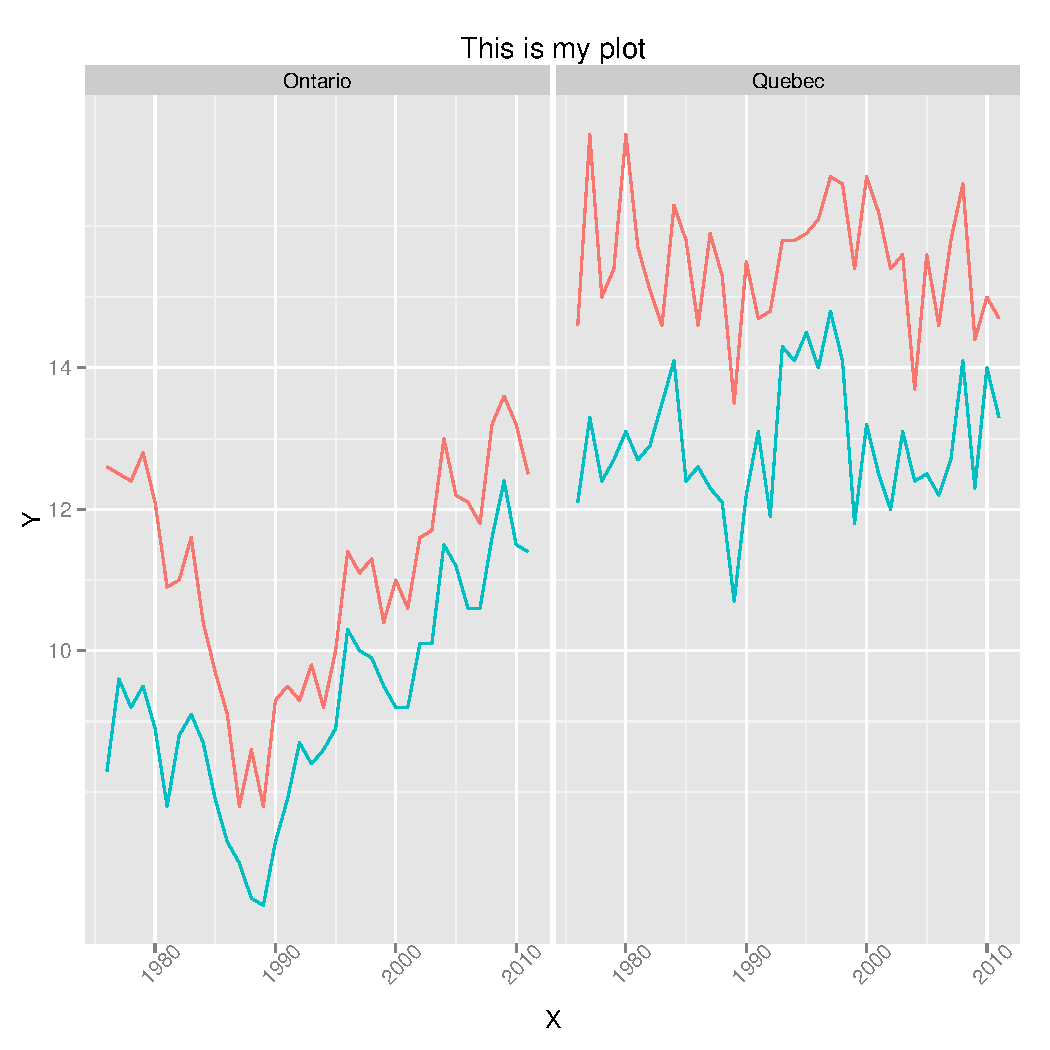
\includegraphics[width=\maxwidth]{figure/unnamed-chunk-11} 

\end{knitrout}

\end{frame}

\begin{frame}
\frametitle{R plot example Cont...}
The last plot is not sized correctly. Playing with the fig.width and fig.height in the chunk options, we can get...
\begin{knitrout}
\definecolor{shadecolor}{rgb}{0.969, 0.969, 0.969}\color{fgcolor}
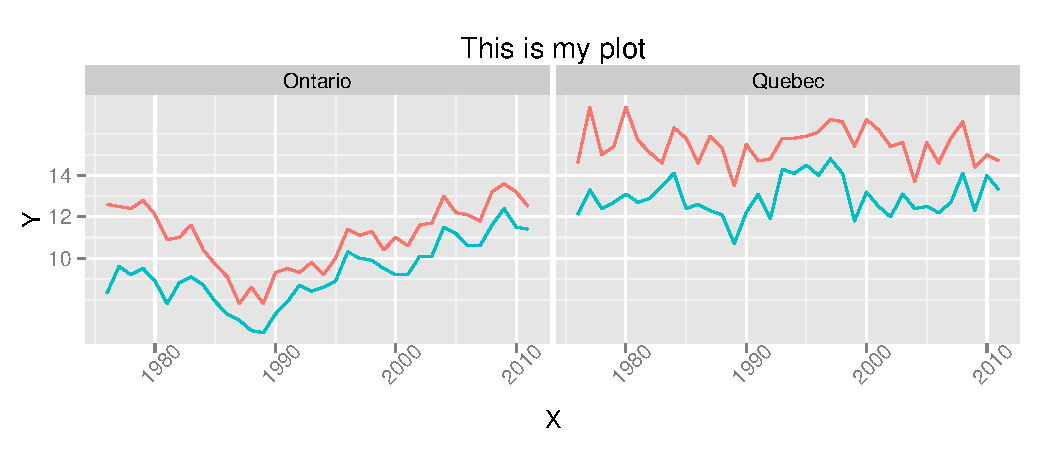
\includegraphics[width=\maxwidth]{figure/unnamed-chunk-12} 

\end{knitrout}

\end{frame}

\begin{frame}[fragile]
\frametitle{Inserting images}
\scriptsize
\begin{itemize}
\item It is very easy to insert images into your frames. To do this, you must load the \textbf{graphicx} package in the preamble.
\item Within a frame environment, use \verb|\includegraphics[options here]{file here}|
\item Ie. \verb|\includegraphics[width=4in]{Picture.pdf}|\\
This gives us the file "Picture.pdf" with a width of 4 inches
\item Alternatively you can use \textbf{scalebox} to shrink a picture to fit the page with \verb|\scalebox{x}{\includegraphics{Picture.pdf}}|
\item Ie. \verb|\scalebox{.5}{\includegraphics{Picture.pdf}}|\\
This gives us the file "Picture.pdf" but shrunk by half
\item The graphic can be in many formats but it is recommended to use .png, .pdf, .eps or .jpg files
\end{itemize}
\end{frame}

\begin{frame}[fragile]
\frametitle{Small tips: Font size and verbatim}
\small
\begin{verbatim}
\tiny, \scriptsize, \footnotesize, \small,
\normalsize, \large, \Large, \LARGE,
\huge & \Huge
\end{verbatim}
These are used to control the font size of the frame. Alternatively you can wrap these commands in \verb|{ }| if you only want to resize a specific line.
Ie. \verb|{\small this is small text}|\vspace{\baselineskip}
\newline Sometimes you want to make sure your text isn't misinterpreted as runnable code. To do this, use the verbatim environment \verb|\begin{verbatim}| and \verb|\end{verbatim}|. \textbf{However}, when using verbatim, you must specify the frame as \emph{fragile}:
\begin{verbatim}
\begin{frame}[fragile]
\end{verbatim}
\end{frame}

\begin{frame}[fragile]
\frametitle{Small tips: supressed captions}
This pertains specifically for article class and not beamer class...Your table captions will be preceded by \textbf{Table 1:} or  \textbf{Table 2:} or whichever table number you are on. You can suppress this by manually writing your caption in latex.\vspace{\baselineskip}
Following a non-floated table (make sure you don't see a \verb|\begin{table}| or \verb|\end{table}| anywhere!), add \verb|\caption{My caption title}| after the \verb|\end{tabular}| commmand. To suppress the numbering, write \verb|\usepackage{caption}| in the preamble and instead of \verb|\caption{My caption title}|, write \verb|\caption*{My caption title}|
\end{frame}

\begin{frame}[fragile]
\frametitle{Why are things going wrong?}
\footnotesize
\begin{itemize}
\item Sometimes your .Rnw will fail to compile. The Log is sometimes not very helpful or specific. So we should go over a few mistakes
\item Sometimes you forget to close an environment. Every line of code: \verb|\begin{}| \textbf{must} be closed by \verb|\end{}| and in correct order.
\item If you have \verb|\begin{document}|, \verb|\begin{frame}|, \verb|\begin{block}|, \verb|\begin{itemize}|, the code must end in the corresponding order" \verb|\end{itemize}|, \verb|\end{block}|, \verb|\end{frame}|, \verb|\end{document}|
\item I recommend testing each frame after completion
\end{itemize}
\end{frame}

\begin{frame}
\frametitle{Anything Else?}
I am not an expert in either LaTeX or Beamer. There are many more features to Ggplot, Sweave and Beamer. Bibtex? Framezoom? Animated graphics? More detail into Hmisc?
\end{frame}

\begin{frame}[fragile]
\frametitle{Additional resources}
\begin{itemize}
\item \url{http://en.wikibooks.org/wiki/LaTeX/Presentations#Columns}
\item \url{http://www.nyu.edu/projects/politicsdatalab/latex/beamer_nyu.pdf}
\end{itemize}
\end{frame}


\end{document}
